%Chapter 3
An explanation of Machine Learning and Neural Networks in general

\section{Autoencoders if they become useful}
Talk about how autoencoders work. Give a nice broad explanation and really go into the math. Include some nice diagrams

Here's \cite{ng2011sparse} a good source to read and model off of. Here \cite{Bhowick2019} is another paper that might be interesting to read. It's about getting noise-free data from the original data using an autoencoder. Neat idea, and could actually be very relevant because they're using geophysical data.

\section{Feed-forward and Backpropagation}

In order to implement a neural network, a solid understanding of linear algebra is needed for the forward pass, whereas backpropagation principally requires vector calculus. Neither action is particularly mathematically complicated; however, there are so many moving parts it is easy to get lost in the sea of similar-sounding partial derivatives. Here, for my benefit, I'm going to walk through the math, as well as the full process of implementing the two function for an affine neural network with 2 hidden layers.

% ## Feed Forward and Einstein Notation

There are enough capital sigmas in the world. I haven't seen anyone use Einstein notation to represent the forward passes of a neural network. Perhaps this is because in practice one usually uses an activation function between each layer.

For a one layer (affine) neural network, the forward propagation is calculated as follows using Einstein notation:

% \begin{figure}[h]
%     \centering
%     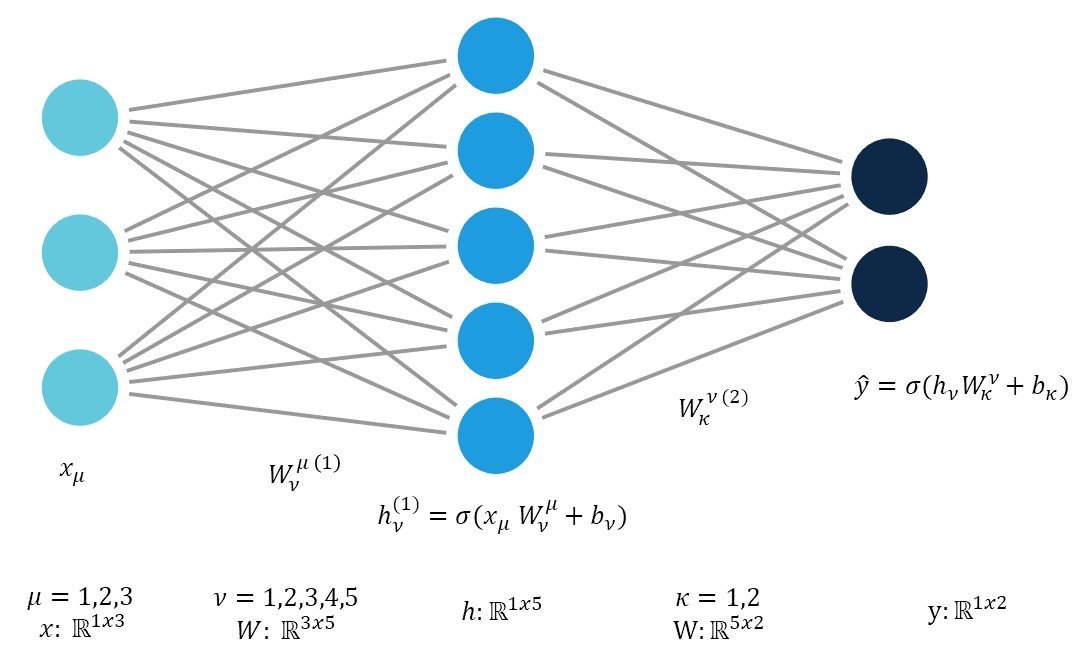
\includegraphics[width=\linewidth]{Chapters/Figures/einstein_NN.png}
%     \caption[Neural Network Example]{Figure first made by me for my website}
% \end{figure}

Recall that repeated indices are implicitly summed over. Explicitly, for one component of the hidden layer:

\begin{align}
    h_j &= \sigma(w_{1j}x_1 + w_{2j}x_2 + w_{3j}x_3 + w_{4j}x_4 + w_{5j}x_5 + b_j) \\
        &= \sigma\Big(\sum_{i=1}^{i=5}w_{ij}x_{i} + b_j\Big)
\end{align}

The process can be repeated ad-nauseam for networks with more layers.

\subsection{Backpropagation}
First, I will show the partial derivative chain rules, and then do it again, more explicitly with defined functions. For now, say your functional is:

\begin{equation}
    \hat{y} = \sigma\left(g\left(f(x,y)\right)\right)
\end{equation}

This would be a network with inputs $(x,y)$, two hidden layer ($ f $  and $ g $ ), and an output with activation function sigma. Lets say the loss is the RMS loss. Thus,

\begin{equation}
    L = \frac{1}{m} \sum (\hat{y} - y)^2
\end{equation}

To see how much we need to shift the weights, we need to find the gradients for each layer. For the first partial derivative, we have:

\begin{equation}
    \frac{\partial L}{\partial L} = 1
\end{equation}

Trivial. Time for the next layer.

\begin{equation}
\frac{\partial \hat{y}}{\partial L} = \frac{\partial L}{\partial L}\frac{\partial \hat{y}}{\partial L}
\end{equation}


It's a little silly to write it this way, but I'm trying to demonstrate a pattern. Next layer:

\begin{equation}
\frac{\partial L}{\partial \sigma} = \frac{\partial L}{\partial \hat{y}} \frac{\partial \hat{y}}{\partial \sigma}
\end{equation}

Next layer:


\begin{equation}
    \frac{\partial L}{\partial g} = \frac{\partial L}{\partial \hat{y}} \frac{\partial \hat{y}}{\partial \sigma} \frac{\partial \sigma}{\partial g}
\end{equation}

Next layer:

\begin{equation}
    \frac{\partial L}{\partial f} = \frac{\partial L}{\partial \hat{y}} \frac{\partial \hat{y}}{\partial \sigma} \frac{\partial \sigma}{\partial g} \frac{\partial g}{\partial f}
\end{equation}

The pattern should be clear. You multiply the gradient calculated in the previous layer by the partial the next layer w.r.t the previous layer.

\subsection{Concrete Example}


